\documentclass{book}
\usepackage{pgf,tikz}
\usetikzlibrary{shapes,arrows,calc,positioning}

% comnado para trazar las rectas verticales dentro de las figuras
% \newcommand*\Paral[2][0.3]{%
%  \draw[thick] ($(#2.north east)-(#1,0)$) -- ($(#2.south east)-(#1,0)$);
%  \draw[thick] ($(#2.north west)+(#1,0)$) -- ($(#2.south west)+(#1,0)$);
% }

\begin{document}

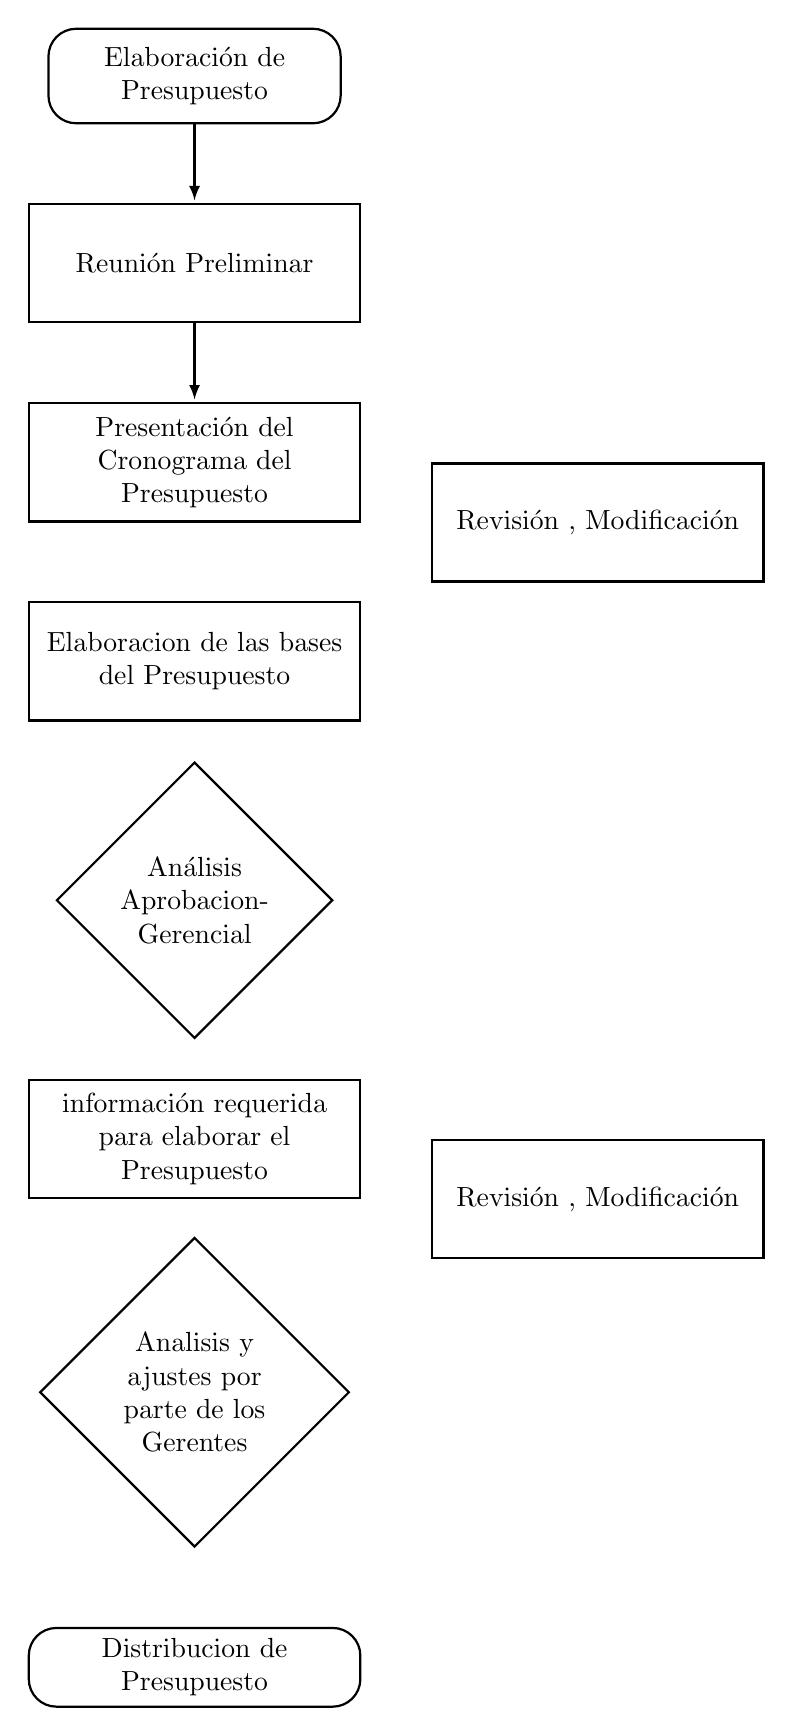
\begin{tikzpicture}
[auto, node distance = 1cm and -1cm,
 every node/.style = {%
  draw = black, thick, fill = white!50,inner sep = 3pt, text badly centered},
 rectangulo/.style = {%
  rectangle, text width=2.5cm, minimum size = 1.5cm},
 rectanguloredo/.style = {rectangle, rounded corners = 10pt},
 line/.style = {draw, thick, -latex,shorten >=1pt},
]

 \node (a) [rectanguloredo, text width=3.5cm, minimum size=1.2cm]
  {Elaboraci\'on de Presupuesto};
 \Paral[0.55]{a}
%  \node (b) [rectangulo, below left=of a] {Presentacion del Cronograma de Presupuestos};
%  \Paral{b} 
 \node (b) [rectangulo, below =of a, text width=4cm] {Reuni\'on Preliminar};
 \Paral{b} 
 \node (c) [rectangulo, below =of b, text width=4cm] {Presentaci\'on del Cronograma del Presupuesto};
 \Paral{c}
 
 \node (d) [rectangulo, below =1cm of c, text width=4cm] {Elaboracion de las bases del Presupuesto};
 
 \node (e) [rectangulo,below= 3.5cm of c ,right =3cm , text width=4cm] {Revisi\'on , Modificaci\'on};
 \Paral{e}
%  \node (e) [rectangulo, below =of c, text width=2.2cm] {informacion requerida para elab el Presupuesto};
%  \Paral{e}
 \node (f) [diamond, below =.5cm of d, text width=2cm] {An\'alisis Aprobacion-Gerencial};
 \Paral{f}
%  \node (g) [regular polygon, regular polygon sides=4, below = of f, text width=1cm] 
%   {Si o no};
 \node (g) [rectangulo, below = .5cm of f, text width=4cm] 
  {informaci\'on requerida para elaborar el Presupuesto };

 \node (h) [diamond, below =2.5cm of f, text width=2cm] {Analisis y ajustes por parte de los Gerentes};
 \Paral{h}
 
 \node (i) [rectangulo, below= of g ,right =3cm , text width=4cm] {Revisi\'on , Modificaci\'on};
 
 \node (j) [rectanguloredo, below = of h, rounded corners = 10pt, text width=4cm,  
  minimum size=1cm] {Distribucion de Presupuesto};
  
% \newdimen\midima
% \pgfextractx{\midima}{(a.south)}
% \newdimen\midimb
% \pgfextractx{\midimb}{(b.north)}
% \newdimen\midimc
% \pgfextractx{\midimc}{(c.north)}
% \newdimen\midimd
% \pgfextractx{\midimd}{(d.west)}
% \newdimen\midime
% \pgfextractx{\midime}{(e.south)}
% \newdimen\midimf
% \pgfextractx{\midimf}{(f.north)}
% \newdimen\midimaw
% \pgfextractx{\midimaw}{(a.west)}
% \newdimen\midimgw
% \pgfextractx{\midimgw}{(g.west)}

 \begin{scope}[every path/.style=line]
 \path
  (a.south) -- ++(0,-0.4) |- ++($(\midimb,0)-(\midima,0)$) -| (b.north);
%  \path
%   (b.south) -- ++(0,-0.4) |- ++($(\midimc,0)-(\midima,0)$) -| (c.north);
 \path (b) -- (c);
%  \path (c) -- (d);

%  \path
%   (d.south) -- ++(0,-0.4) |- ++($(\midimd,0)-(\midimf,0)$) -| (f.east);

%  \path
%   (e.south) -- ++(0,-0.4) |- ++($(\midime,0)-(\midimf,0)$) -| (f.north);
%   \path (d.south) -- (f.east);
%  \path (f) -- (g);
%  \path (g.west) node[draw = none, fill = none, yshift = 0.3cm, xshift = -0.4cm] {text} 
%   -- ++(-3.5,0) -- ++($(0,\midimaw)-(0,\midimgw)$) |- (a);
%  \path (g) -- node[draw = none, fill = none, xshift = 0.1cm] {text} (h);
 \end{scope}
\end{tikzpicture}

\end{document}